\section{Filter}\label{sec:filter_design}

The aim of this chapter is to analyse the data from \ref{sec:opt_result} and choose the implementation method. From the beam forming optimization \autoref{sec:genetic_con} it was concluded that there shall be a cost filter and a beam forming filter. This chapter starts analyse the cost filter and design a filter solution, then the beam forming filter will be analysed and a solution will be designed.


\section{The cost filter}
The analysis of the cost filter will be done only with respect to the gain of the transfer function and without taking the phase intro account. The reason to avoid the phase is that the filter is an input filter to the entire system, and therefore the phase of the filter will affect all speaker the same way and therefore not effect the beam forming. \\
To analyse the cost filter, the filter type and the slope or Q of the filter have to be determined. 

the filter type will be determined first. To determined the filter type, a second order polynomia estimation will be done on the data point of the cost filter. The polynomia estimation is done with MATLAB command \texttt{polyfit()} with a second order regression. This give a second order polinomia where  \texttt{polyval()} is used to estimate the filter transfer function. The estimation will be done from \SI{60}{\hertz} to \SI{400}{\hertz}. The \SI{400}{\hertz} choice is made such that the estimation fit at lest to the double frequency of beam forming interest. The following \autoref{} shows the estimate compare to the original data point.

\begin{figure}[H]
	\centering
	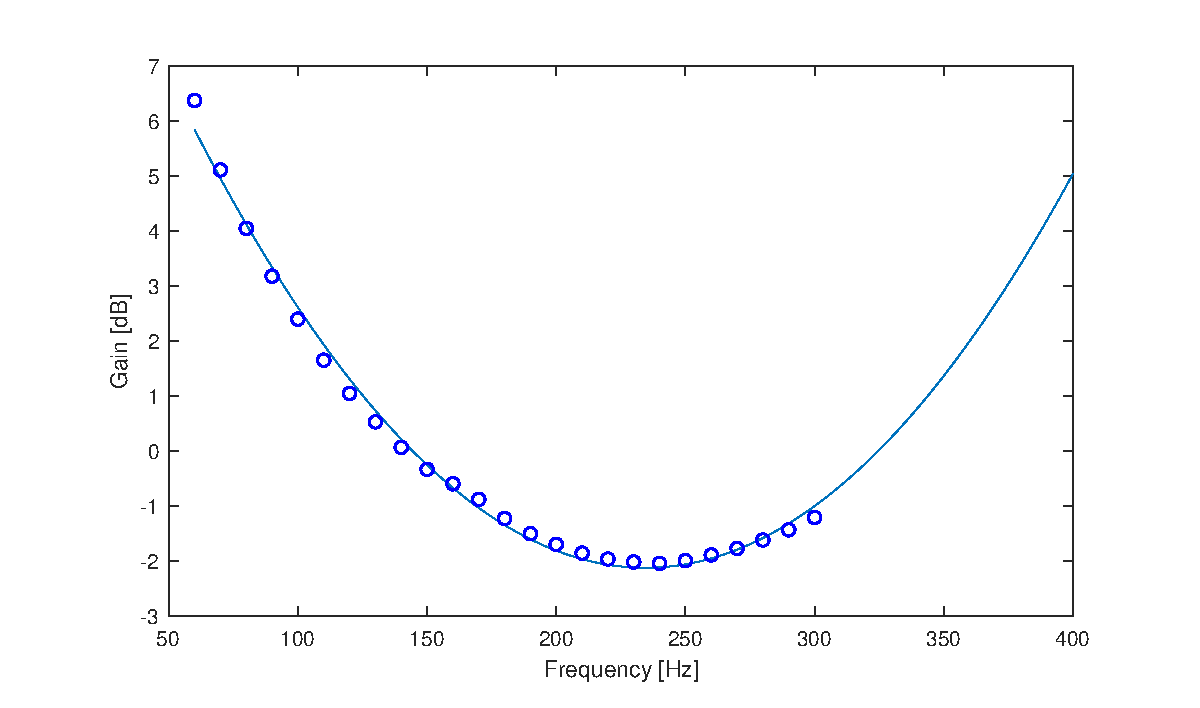
\includegraphics[width=1\textwidth]{band_stop_filter.eps}
	\caption{The graph shows transfer function of the estimated transfer function, where the blue  Solid line is the gain. All circle in the graph is the actual optimized point.}
		\label{fig:band_stop_filter}
\end{figure}


As it can be seen on \autoref{band_stop_filter} the shape of the estimated cost filter is a band stop filter with a relative gain of \SI{8.5}{\decibel}, and have a center frequency of \SI{175}{\hertz}. There needs to be a gain factor before the filter, to achieve the wanted band stop filter. The gain in the front of the filter will need to be \SI{6.4}{\decibel}. \\

\subsection{Band pass filter}

Designing a bandstop filter is done with designing it as a band boost filter and then change the filter from feed forward to feedback coupled filter. Thats mean that the filter will be change to following \autoref{fig:band_pass_filter}


\begin{figure}[H]
	\centering
	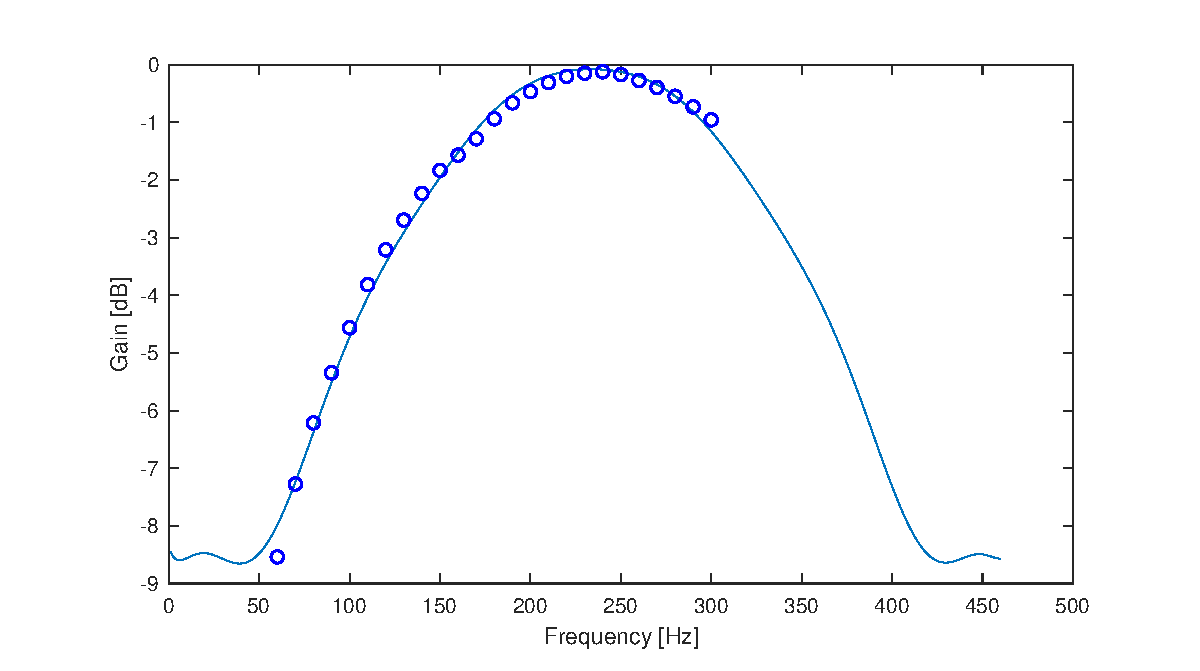
\includegraphics[width=1\textwidth]{band_pass_filter.eps}
	\caption{The graph shows transfer function of the estimated transfer function, where the blue  Solid line is the gain. All circle in the graph is the actual optimized point.}
		\label{fig:band_pass_filter}
\end{figure}

It can be seen on the figure, that the \SI{-3}{\decibel} bandwidth is \SI{213}{\hertz}, a center frequency of \SI{234}{\hertz} the gain must be \SI{8.5}{\decibel} 


\begin{figure}[H]
	\centering
	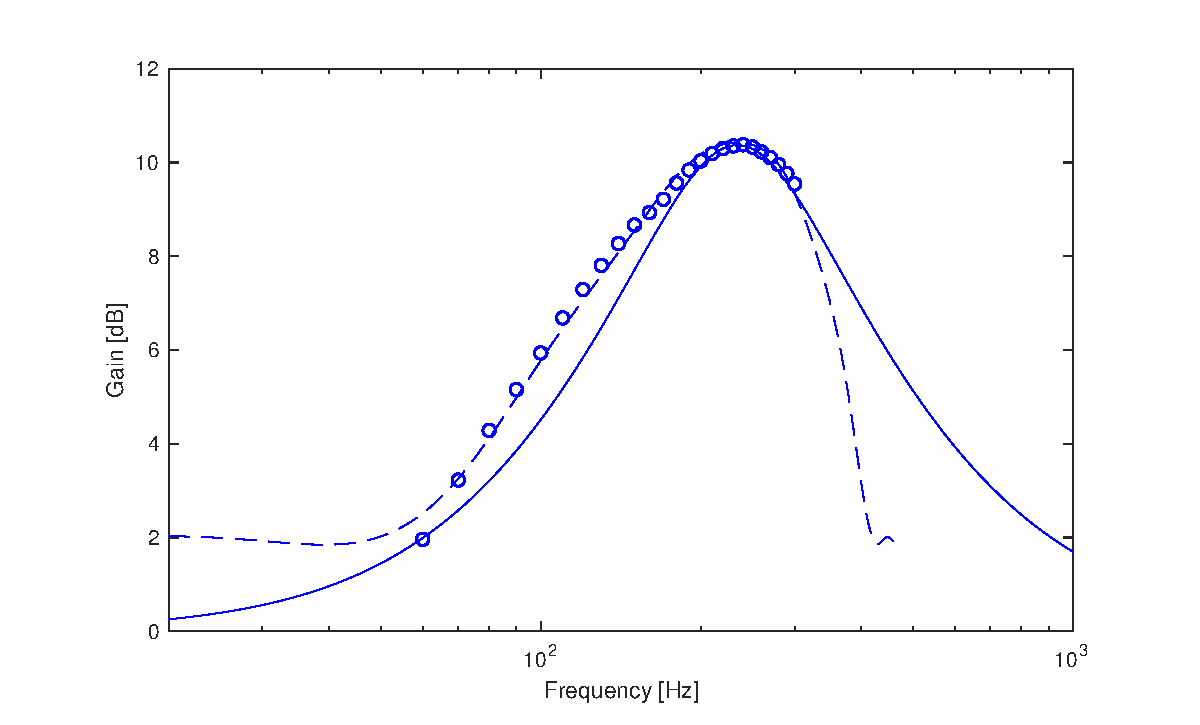
\includegraphics[width=1\textwidth]{band_pass_filter_h_non_scaled.eps}
	\caption{The graph shows transfer function of the estimated transfer function, where the blue  Solid line is the gain. All circle in the graph is the actual optimized point.}
		\label{fig:band_pass_filter_h_non_scaled}
\end{figure}

The wanted filter is raised by \SI{2}{\decibel} such that the designed filter also fit at low frequency. The output of the filter shall afterwards by atunuated by  \SI{2}{\decibel} to work as wanted.


It can be seen on \autoref{fig:band_pass_filter_h_non_scaled} that the \SI{-3}{\decibel} bandwidth is to narrov because the wanted filter have symmetrical shape in linear domain and not in logorithmic doman which the filter have.Therefore the filter bandwidth have to be extended with a factor of 1.1878. The factor is founded by trail and error. After the bandwidth is extended the filter is as following \autoref{fig:band_pass_filter_h}


\begin{figure}[H]
	\centering
	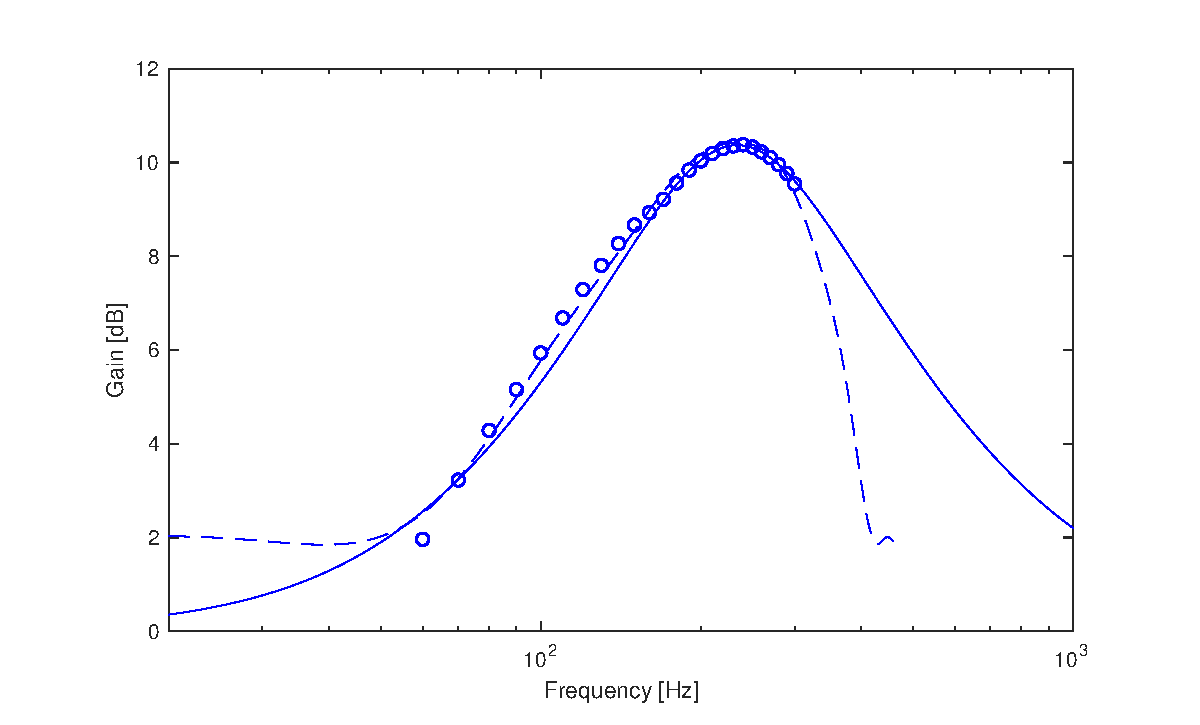
\includegraphics[width=1\textwidth]{band_pass_filter_h.eps}
	\caption{The graph shows transfer function of the estimated transfer function, where the blue  Solid line is the gain. All circle in the graph is the actual optimized point.}
		\label{fig:band_pass_filter_h}
\end{figure}


\subsection{Band stop filter form second order filter}
To transform a band pass filter to a band stop filter which not is a notch filter, the filter have to be transformed from a feed forward filter to a feedback filter 


(BLOCK DIAGRAM)

To transform the bandpass filter to a bandstop filter as descriped above, only the denominator and the numerator have to be switch around.

(The new formula)


\begin{figure}[H]
	\centering
	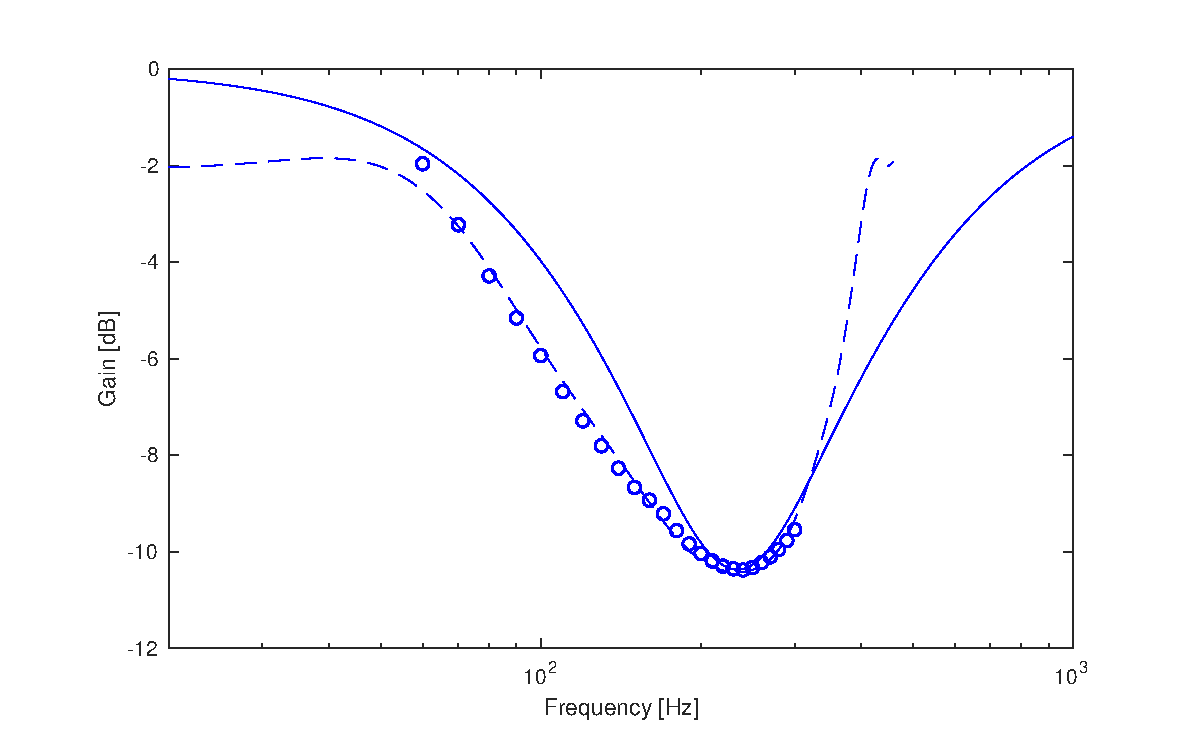
\includegraphics[width=1\textwidth]{band_stop_filter_non_scaled.eps}
	\caption{The graph shows transfer function of the estimated transfer function, where the blue  Solid line is the gain. All circle in the graph is the actual optimized point.}
		\label{fig:band_stop_filter_non_scaled}
\end{figure}


\begin{figure}[H]
	\centering
	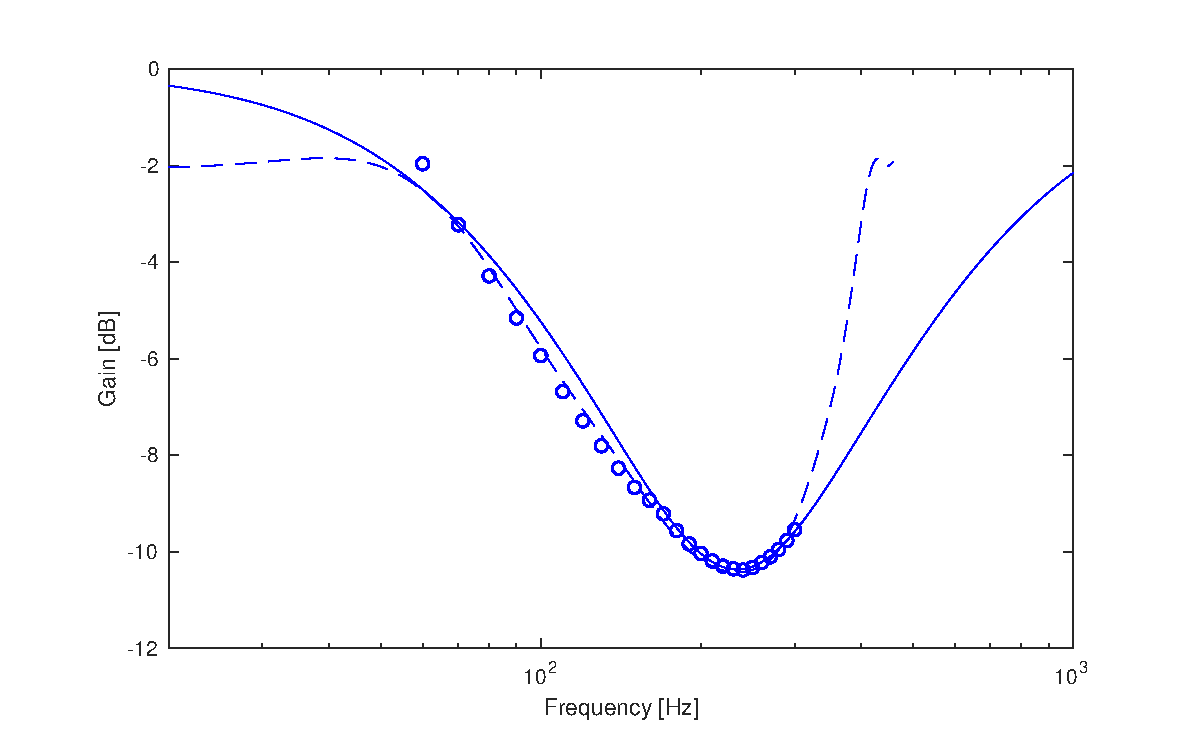
\includegraphics[width=1\textwidth]{band_stop_filter_scaled.eps}
	\caption{The graph shows transfer function of the estimated transfer function, where the blue  Solid line is the gain. All circle in the graph is the actual optimized point.}
		\label{fig:band_stop_filter_scaled}
\end{figure}


 The second step is to find the slope of the needed low pass filter. The slope is founded as following \autoref{eq:filter_slope}

\begin{equation}
\text{slope} = \frac{G_2\si{\decibel}-G_1\si{\decibel}}{\log_{10}{(f_2)}-\log_{10}{(f_1)}}
\end{equation}

    \startexplain
    \explain{$f$ is a frequency point }{\si{\hertz}}
    		\explain{$f_2$ is a frequency point higher that $f_1$ }{\si{\meter}}
        \explain{$G_1\si{\decibel}$ is the corresponding amplitude to $f_1$}{\si{\decibel}}
         \explain{$G_2\si{\decibel}$ is the corresponding amplitude to $f_2$}{\si{\decibel}}
    \stopexplain
    
The calculated slope is $17 \frac{\si{\decibel}}{dec}$ and it have been chosen that a standard first order low pass filter will be used. The following \autoref{} shows the error between the data and the filter. The error will make a pressure deference, that defence on frequency. 


\section{Beam forming filter}
The beam forming filter is not as easy as the cost filter to design, since that the phase and the gain have to be exact before the beam forming works. Therefore the phase have to be studied to determined the filter type. On the data point from the \ref{sec:opt_result} it can be seen that the phase is mostly linear in the frequency of interest, and therefore the filter will be a linear phase \gls{fir} filter. The smart thing with choosing a \gls{fir} filter is that the impulse response of the filter just have to be symmetric to achieve linear phase response. This means that optimizing the part of the impulse response and put it together with a mirrored version will always achieve linear phase. One disadvantages is that the cut off frequency is in the low frequency and therefore the filter order have to be high. \\

 A modified version of the genetic optimization algorithm will be used to find a optimized impulse response of the filter. To optimize the impulse respond of the filter, an estimate of the impulse respond have to be determined. One and the used way to estimate the impulse response is to transfer all polar coordinate to a complex rectangular transfer function and take the real of the \gls{ifft} of the complex transfer function. The polar to rectangular transform is done as following \autoref{eq:pol_to_regt}

\begin{equation}\label{eq:pol_to_regt}
x=rcos(\phi)+j \cdot rsin(\phi)
\end{equation}


     \startexplain
    \explain{$\phi$ is the angle of the transfer function in radian }{\si{1}}
        \explain{$r$ is the amplitude of the transfer function}{\si{1}}
        \explain{$j$ is the imaginary unit}{\si{1}}
    \stopexplain

The real of the \gls{ifft} gives an estimated impulse response but with a scaled cross over point. The meaning with scaled cross over point is that the cross over point follows the scaling of the sample frequency. With a sample rate of \SI{44.1}{\kilo\hertz} the following  \autoref{} shows the transfer function of the estimated impulse response. 

\begin{figure}[H]
	\centering
	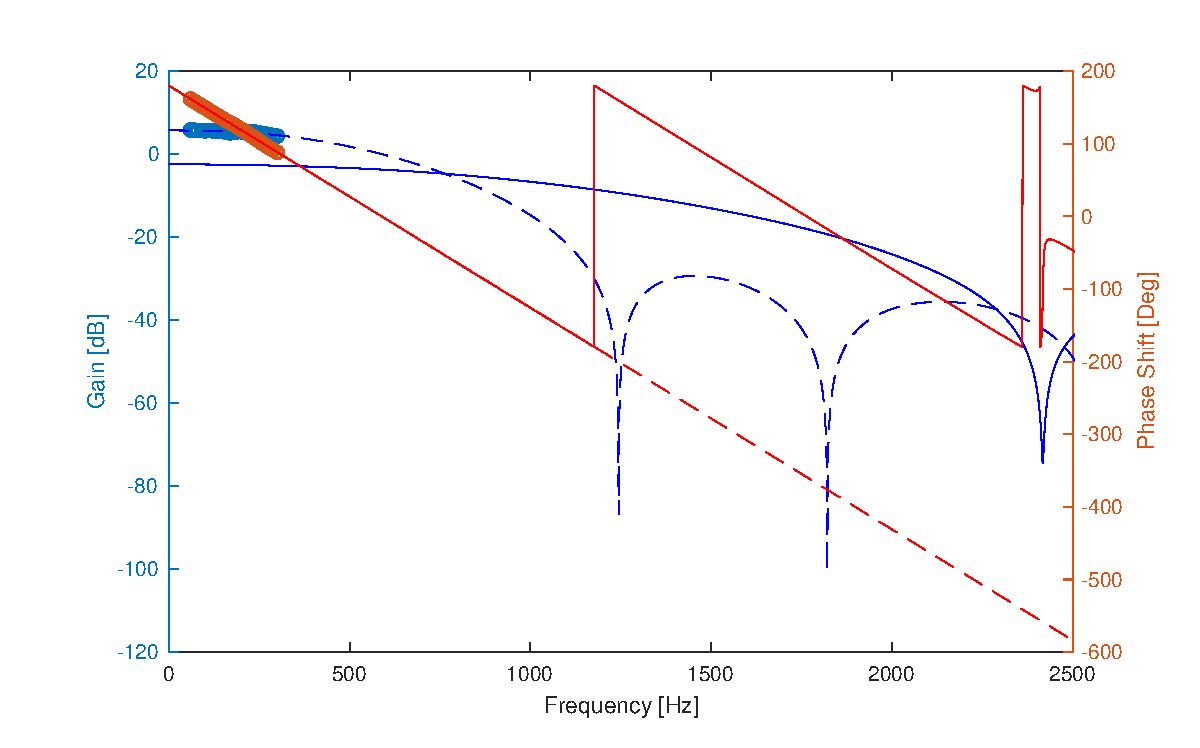
\includegraphics[width=1\textwidth]{ir_estimate_non_scaled.eps}
	\caption{The graph shows transfer function of the estimated impulse respond. The dashed line is transfer function that is needed for beam forming filter, where the blue line is the gain and the red line is the phase. The Solid line line is the transfer function of the estimated impulse response, where the blue line is the gain and the red line is the phase. All circle in the start of the graph is the actual optimized point.}
		\label{fig:ir_estimate_non_scaled}
\end{figure}


It can be seen that the cross over lays at a too high frequency and the gain at the frequency of interest is to low. The corresponding impulse response of the transfer function in \autoref{fig:ir_estimate_non_scaled} is as following \autoref{fig:ir_estimate_non_mirror} where the mirrored version not is added yet. 

\begin{figure}[H]
	\centering
	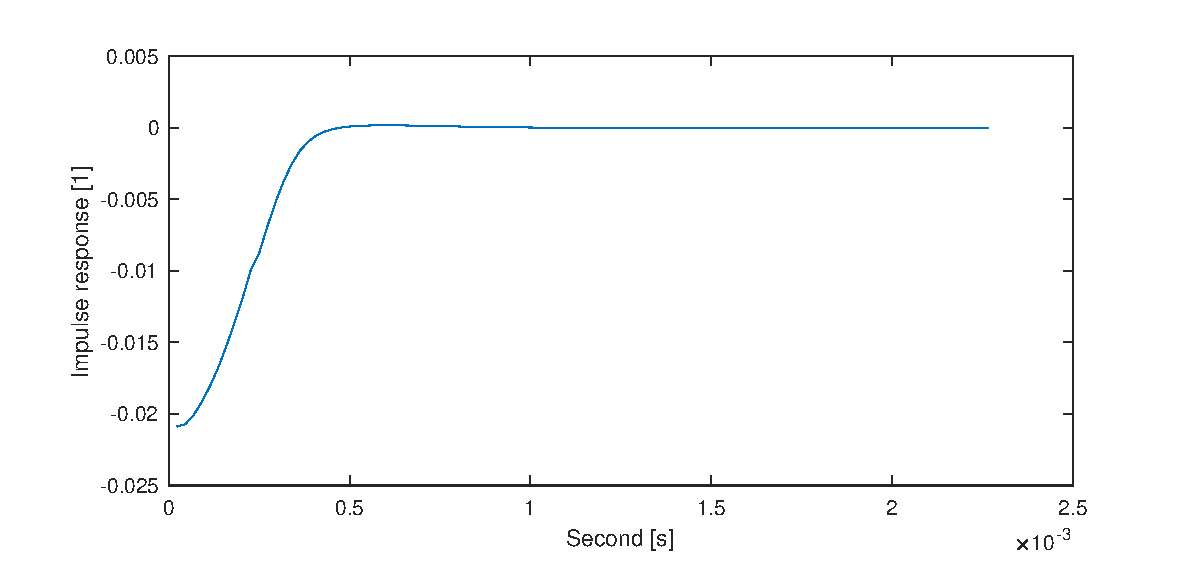
\includegraphics[width=1\textwidth]{ir_estimate_non_mirror.eps}
	\caption{The graph shows the impulse respond where the mirrored version is added to the impulse respond}
		\label{fig:ir_estimate_non_mirror}
\end{figure}

The version where the mirrored impulse response is added to the impulse response and the phase is matched to the wanted phase and is the corresponding impulse response to \autoref{fig:ir_estimate_non_scaled} is \autoref{fig:ir_estimate_mirror}

\begin{figure}[H]
	\centering
	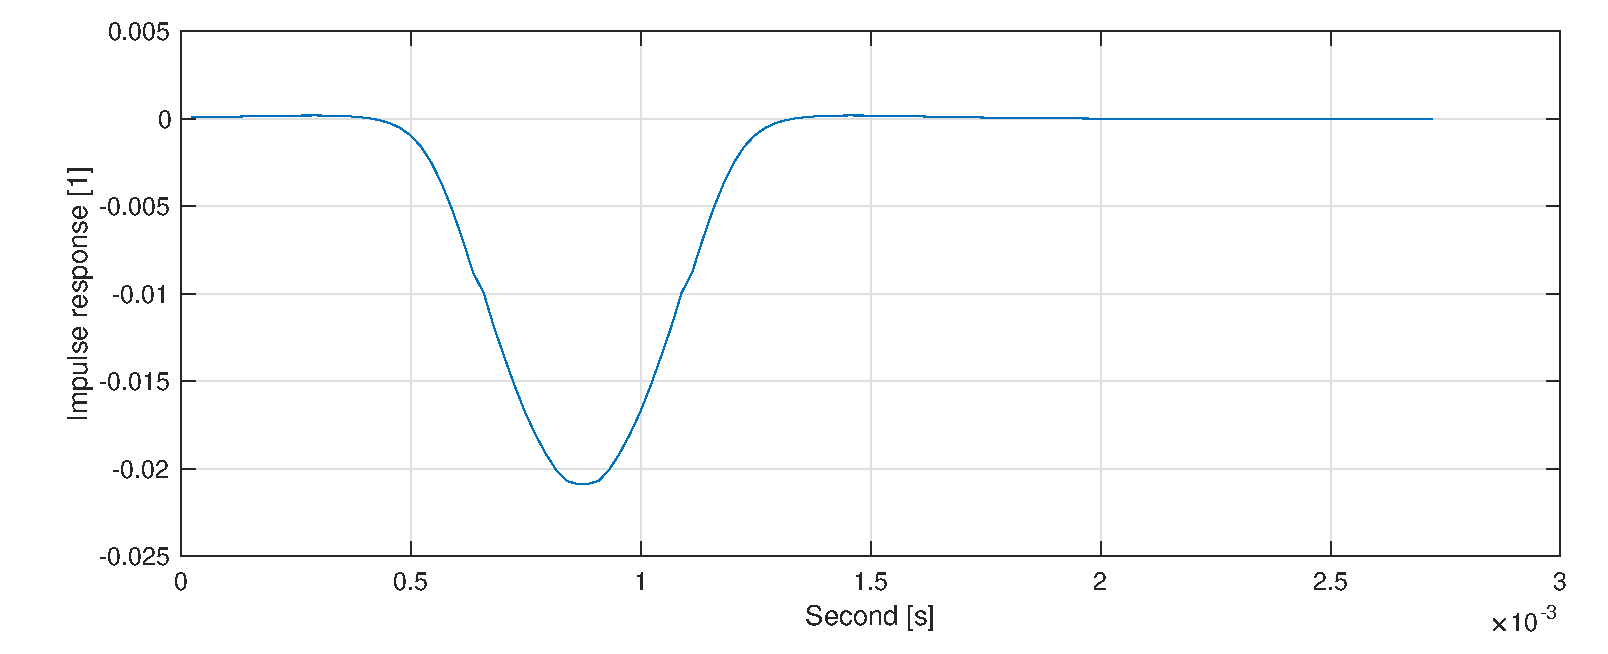
\includegraphics[width=1\textwidth]{ir_estimate_mirror.eps}
	\caption{The graph shows the impulse respond where the mirrored version is added to the impulse respond}
		\label{fig:ir_estimate_mirror}
\end{figure}


The impulse response have to be change the right way to make a good estimate. The way to lower the cross over point is to extend the part of the impulse respond that it have the highest amplitude, which also make the impulse response longer. Thinking about the theory of the \gls{fir} filter, that the lower cross over, the higher order the filter have to be and therefore the impulse respond gets longer. The following \autoref{} shows the estimated impulse respond that will be used for the optimization, where the crossover is approximatly where it shall be. 


\begin{figure}[H]
	\centering
	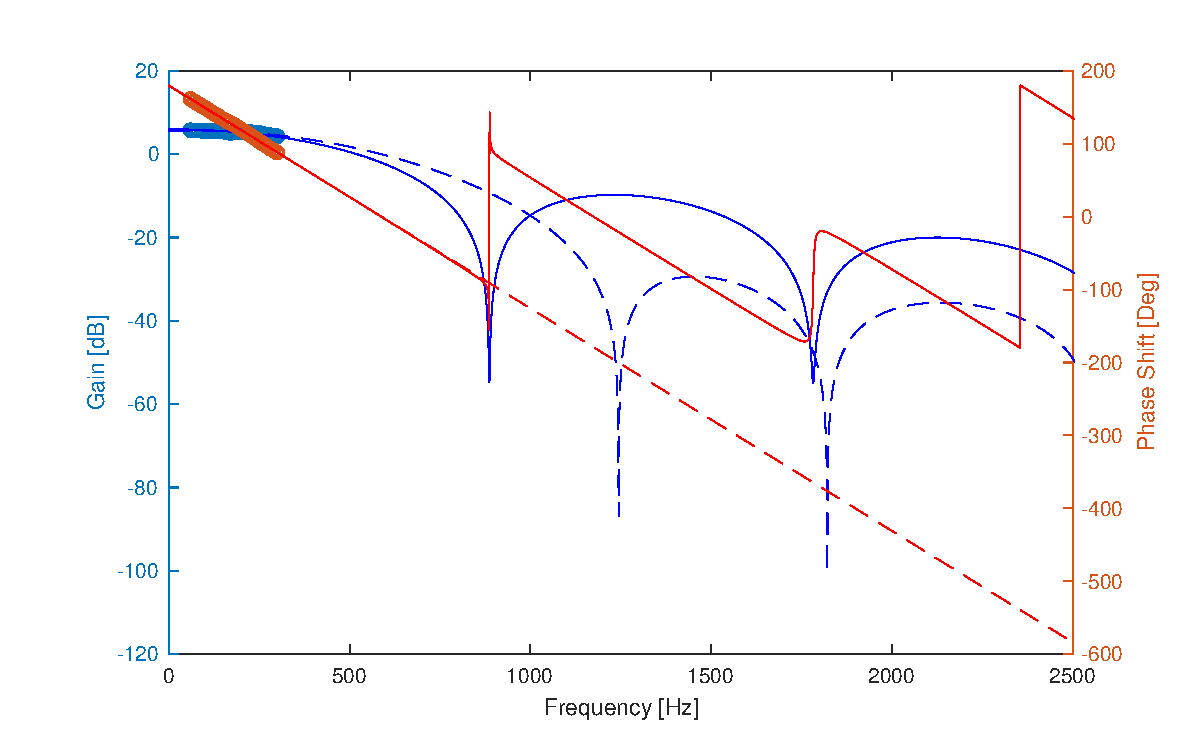
\includegraphics[width=1\textwidth]{ir_estimate_scaled.eps}
	\caption{The graph shows transfer function of the estimated impulse respond. The dashed line is transfer function that is needed for beam forming filter, where the blue line is the gain and the red line is the phase. The Solid line line is the transfer function of the estimated impulse response, where the blue line is the gain and the red line is the phase. All circle in the start of the graph is the actual optimized point.}
		\label{fig:ir_estimate_scaled}
\end{figure}

Where the corresponding impulse response is as \autoref{fig:ir_estimate_mirror_scale}


\begin{figure}[H]
	\centering
	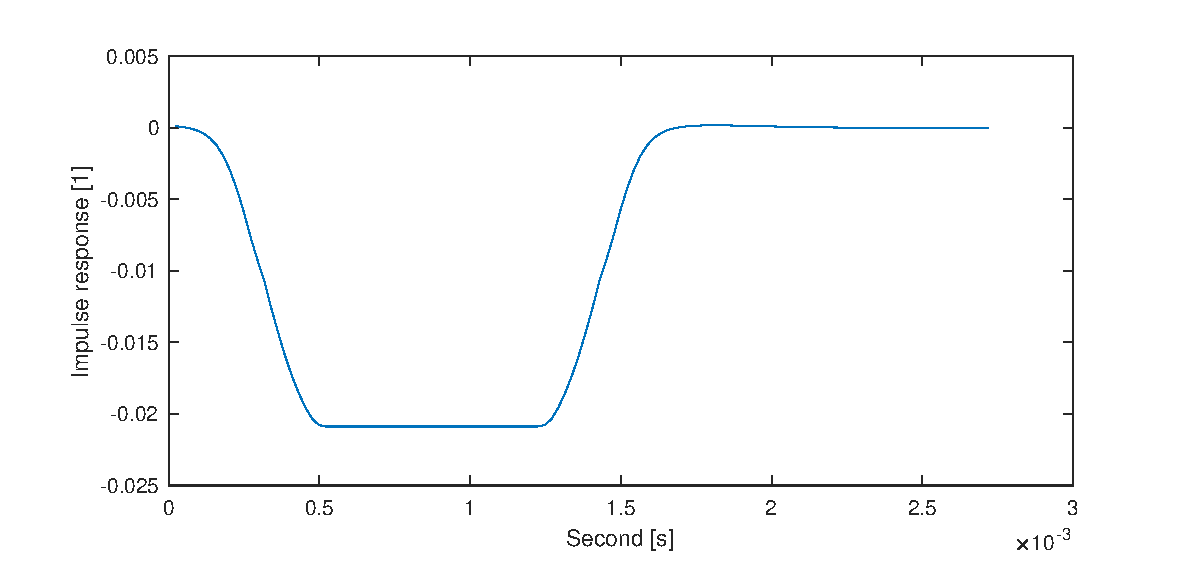
\includegraphics[width=1\textwidth]{ir_estimate_mirror_scale.eps}
	\caption{The graph shows the impulse respond where the mirrored version is added to the impulse respond}
		\label{fig:ir_estimate_mirror_scale}
\end{figure}

As it can be seen at \autoref{fig:ir_estimate_scaled} that the cut off is lowered and the gain is automatic raised to the wanted area. A closer look on the area of the frequency of interest in 

\begin{figure}[H]
	\centering
	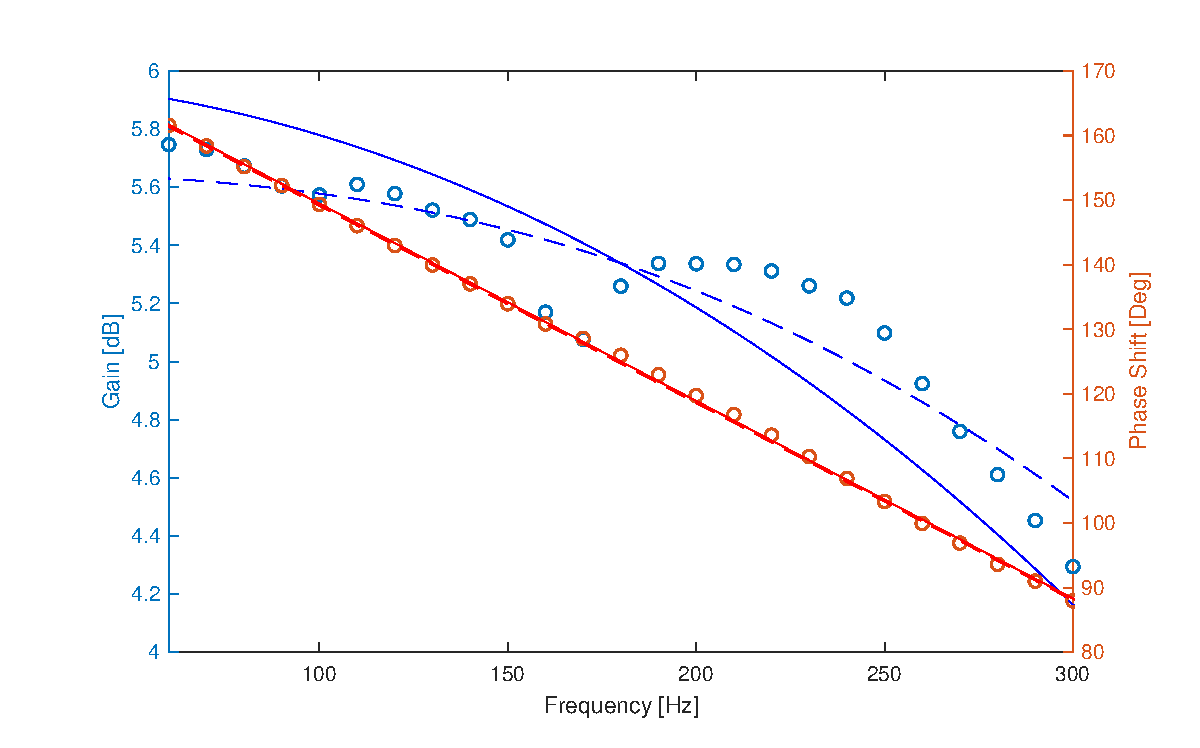
\includegraphics[width=1\textwidth]{ir_estimate_scaled_close.eps}
	\caption{The graph shows transfer function of the estimated impulse respond. The dashed line is transfer function that is needed for beam forming filter, where the blue line is the gain and the red line is the phase. The Solid line line is the transfer function of the estimated impulse response, where the blue line is the gain and the red line is the phase. All circle is the actual optimized point.}
		\label{fig:ir_estimate_scaled_close}
\end{figure}

It can be seen at \autoref{ir_estimate_scaled_close} that the fit is close, but the gain can be optimized. Recalling from earlier, a linear phase \gls{fir} filter have to have symmetric impulse response and therefore the impulse respond where the mirrored version is not added will be used as initial guess for the genetic optimizer. To optimize the impulse response there will be used high probability for mutation and crossover. The resend to use high probability for mutation, is that the shape of the impulse response is changed a bit for every mutation, and it is the shape there needs to be change to get the optimized \gls{fir} filter coefficient. In the mutation part, the following mutation is done.

\begin{itemize}
\item One single random chosen point in the impulse response is change by moving it up and down wards.
\item One random chosen area of the impulse response is change by moving it up and down wards with a Gaussian shape, where $\mu$ and $\sigma$ is random chosen.
\item An up-sampling is done on the impulse respond with a factor of ten. After the up-sampling the value at time zero is copied and used ans the new zero point after the impulse response is shifted one sample to the right. The resend to up-sample is that the shift only is one tenth. This technique do that the cost can be minimized more than without up-sampling. The up-sampling is done with linear interpolation. This mutation ends with a down sampling with a factor of ten such that the impulse respond is at the same length as at the start.
\item There is one mutation that only multiply a factor to the impulse respond. 
\end{itemize}

At the end of all mutation the last point of the impulse response is used as the \gls{dc} offset and the offset will be subtracted from the impulse response , such that the impulse response end at an amplitude of zero. 




 



